\chapter{The Transport Equation}

In this lecture, we introduce general \textit{transport equations} and finish by developing the form used in neutron transport theory.  In the lectures to follow, we shall describe other aspects of the neutron transport equation and methods by which it can be solved both analytically and numerically.

\section*{Transport Theory}

Transport theory aims to describe mathematically the movement (i.e. ``transport'') of particles as they traverse a medium.  For example, we might describe the transport of high energy gammas through a lead shield, or the movement of neutrons through uranium dioxide pellets.  We might also describe the movement of particles in a dense gas as they navigate through a medium consisting of the gas itself.

In all cases, transport theory describes such processes in an \textit{average} sense.  For instance, we do not compute the individual trajectories of neutrons in a reactor via transport theory.  That, instead, would require molecular dynamics, in which Newton's equation of force is solved for the many-bodied problem of all neutrons in the vicinity of interest (an essentially impossible problem), or perhaps the Monte Carlo methods described in previous lectures, where a sample of individual particles are tracked to approximate ensemble averages (a difficult, but as we've seen, tractable problem).  Hence, the quantities we shall compute using the equations of transport theory should be recognized as expected and not exact values.

\section*{Fundamental Quantities}

We begin by defining several fundamental quantities.  It should be noted that the forms introduced at first are likely different from what you might have seen in a previous reactor physics course.  The purpose here is two-fold.  First, we wish to introduce the quantities and eventually the equations in a general way to make clear that transport theory is not restricted to the neutron transport equation.  Second, for those who might be familiar with e.g. the Boltzmann equation of gas dynamics (and not neutron transport), the notation will be familiar and lead smoothly into our more familiar form.

We first define the \textit{phase space density function}, the knowledge which we can use to compute essentially all quantities of interest:
\begin{center}
  \begin{tabular}{cp{7.0cm}}
    $n(\mathbf{r},\mathbf{v},t)d^3r d^3v \equiv $ &
    expected number of particles in  $d^3r$  about  $\mathbf{r}$  with velocity  $dv$ about  $\mathbf{v}$ at time $t$.  
  \end{tabular}
\end{center}
It is often most convenient to break the velocity into its scalar (speed) and vector (direction) components.  The scalar component is recast in the energy variable via $E = mv^2/2$, and the direction vector is defined $\mathbf{\Omega}=\mathbf{v}/|\mathbf{v}|$.  The phase space density can then be rewritten as
\begin{center}
  \begin{tabular}{cp{7.0cm}}
    $n(\mathbf{r},\mathbf{\Omega},E,t)d^3r d\Omega dE \equiv $ &
    expected number of particles in  $d^3r$  about  $\mathbf{r}$  going in the directions $d\Omega$ about $\mathbf{\Omega}$ with energy  $dE$ about  $E$ at time $t$.  
  \end{tabular}
\end{center}
In this form, $n(\mathbf{r},\mathbf{\Omega},E,t)$ is often referred to as the angular density.

\begin{wrapfigure}{r}{0.5\textwidth}
    \begin{center}
    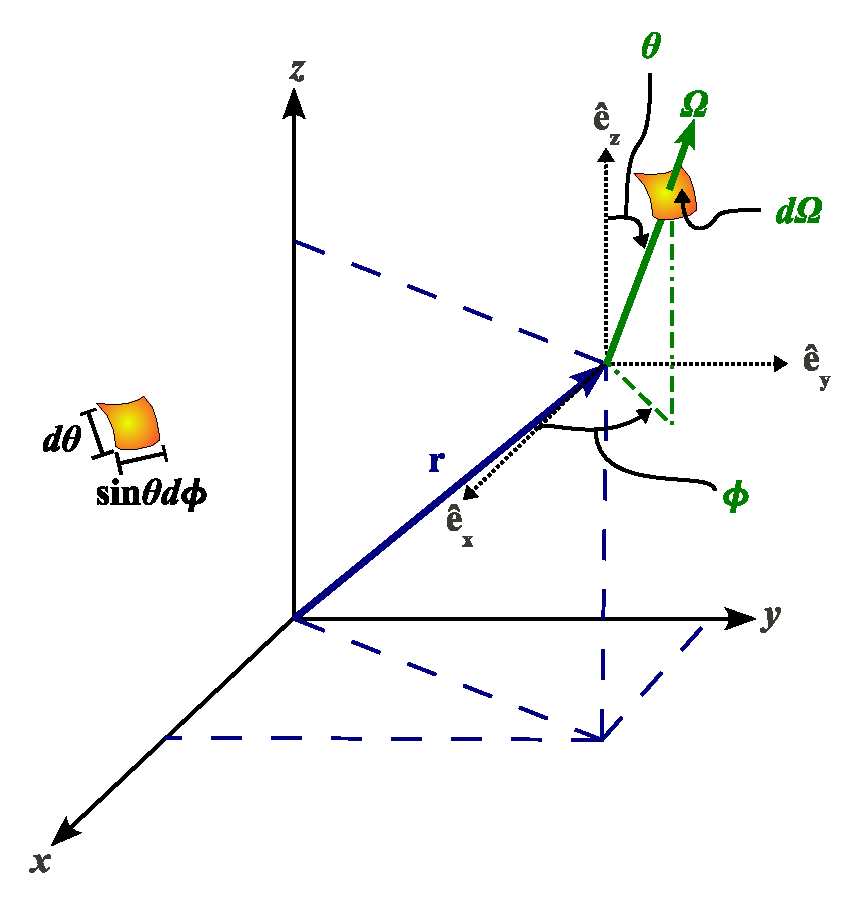
\includegraphics[keepaspectratio, width = 2.7 in]{images/phase_space}
    \end{center}
    \caption{Schematic of Phase Space.}
    \label{fig:phase_space}
\end{wrapfigure}

We can relate the phase space densities in terms of $\mathbf{v}$ and $(E,\mathbf{\Omega})$ via the relations
\begin{equation}
 \begin{split}
  n(\mathbf{r},E,\mathbf{\Omega},t) &= (v/m) n(\mathbf{r},\mathbf{v},t) \\
  n(\mathbf{r},E,\mathbf{\Omega},t) &= (1/mv) n(\mathbf{r},v,\mathbf{\Omega},t) \\
  n(\mathbf{r},v,\mathbf{\Omega},t) &= v^2 n(\mathbf{r},\mathbf{v},t) \, ,
 \end{split}
 \label{eq:densityrelations}
\end{equation}
proofs of which are left as exercises.

Figure \ref{fig:phase_space} depicts a schematic of the phase space used in terms of the position $\mathbf{r}$ and direction $\mathbf{\Omega}$.  The position vector is further broken down into the polar angle $\theta$ and azimuthal angle $\phi$.  The differential solid angle element $d\Omega$ is also shown, and can be expressed in terms of $\theta$ and $\phi$ via
\begin{equation*}
 d\Omega = \sin{\theta} d\theta d\phi \, .
\end{equation*}  
One might envision such solid angle elements as the small bumps on basketballs.  

A quantity closely related to the phase space density (or current density) is the \textit{angular current density}:
\begin{center}
  \begin{tabular}{cp{5.0cm}}
    $\mathbf{j}(\mathbf{r},\mathbf{v},t)\cdot d\mathbf{S} d^3v = \mathbf{v} n(\mathbf{r},\mathbf{v},t) \cdot d\mathbf{S} d^3v \equiv $ &
    expected number of particles that cross an area $dS$ per second with velocity $d^3v$ about $\mathbf{v}$ at time $t$.
  \end{tabular}
\end{center}

We can also define \textit{partial currents} with respect to a particular surface $S$ defined by an outward normal vector $\mathbf{\hat{e}}_s$:

\begin{center}
  \begin{tabular}{cp{5.0cm}}
    $J_{\pm}(\mathbf{r},t) = \pm \int_{\pm} d^3v  \mathbf{\hat{e}}_s \cdot \mathbf{j} (\mathbf{r},\mathbf{v},t) \equiv $ &
   the rate at which particles flow through $S$ in the outward (+) or inward (-) direction.
  \end{tabular}
\end{center}

The \textit{current density} $\mathbf{J}(\mathbf{r},t)$ is defined by integrating the angular current density over all velocities.  Then for our surface $S$, the net rate of particles passing outward through $S$ is just $\mathbf{J}(\mathbf{r},t) \cdot \mathbf{\hat{e}}_s$.  From our definition of partial currents, the net current passing outward must also be $J_+ - J_-$, yielding the useful identity
\begin{equation}
 \mathbf{J}(\mathbf{r},t) \cdot \mathbf{\hat{e}}_s = J_{+}(\mathbf{r},t) - J_{-}(\mathbf{r},t) \, .
 \label{eq:net2partial}
\end{equation}

%A point of caution: it should be noted that $n$ and $\mathbf{j}$ must have the same units but represent wholly different things since $n$ is a scalar quantity while $\mathbf{j}$ is a vector quantity.  This will be true also of $\mathbf{J}$ and the scalar flux $\phi$, which will be introduced

Of particular interest to us in the next section will be reaction rates, which can most easily be described using the \textit{angular flux}
\begin{center}
  \begin{tabular}{cp{2.0cm}}
    $ \psi (\mathbf{r},\mathbf{\Omega},E,t) = v n(\mathbf{r},\mathbf{\Omega},E,t) \equiv $ &
    angular flux
  \end{tabular}
\end{center}
and \textit{scalar flux}
\begin{center}
  \begin{tabular}{cp{2.0cm}}
    $ \phi (\mathbf{r},E,t) = \int_{4\pi} d\Omega \psi (\mathbf{r},\mathbf{\Omega},E,t)  \equiv $ &
    scalar flux.
  \end{tabular}
\end{center}

\section*{A General Transport Equation}

Consider an arbitrary volume $V$ with a surface $S$.  Our goal is to represent the time rate of change of the particle density $n(\mathbf{r},\mathbf{v},t)$ within the volume.  Neglecting external forces, the only factors affecting the density are collisions within the volume that change a particle's velocity, the streaming of particles into and out of the surface, and any internal source of particles.  This simple balance can be expressed mathematically as
\begin{equation}
\begin{split}
 \overbrace{ \frac{\partial}{\partial t} \Bigg ( \int_V d^3 r n(\mathbf{r},\mathbf{v},t) \Bigg ) }^{\text{total rate of change of }n\text{ in } V} 
      &=  - \overbrace{\int_S dS \mathbf{\hat{e}}_S \cdot \mathbf{j}(\mathbf{r},\mathbf{v},t) }^{\text{streaming rate}}
       + \overbrace{ \int_V d^3 r \Big( \frac{\partial n}{\partial t} \Big )_{\mathrm{coll}} }^{\text{collision rate}} \\
      &+ \underbrace{ \int_V d^3 r s(\mathbf{r},\mathbf{v},t) }_{\text{source emission rate}}  \, ,
\end{split}
\label{eq:balance}
\end{equation}
where $s$ represents a source inside the volume and $(\partial n/\partial t)_{\mathrm{coll}}$ is the time rate of change due to collisions, specific forms of which are application-dependent and will be discussed below.  Note the minus sign on the surface integral, i.e. the streaming term.  Since the integral describes the net rate of neutrons going \textit{out} of the surface, we negate it so that a positive net rate directed inward is a positive contribution to the total time rate of change of $n$ in $V$.

Eq. \ref{eq:balance} gives us a simple relation in terms of both volume and surface integrals.  Our life is always easiest if we have the same integration on both sides.  By the divergence (or Gauss') theorem, we can rewrite the streaming term
\begin{equation}
 \int_S dS \mathbf{\hat{e}}_S \cdot \mathbf{j}(\mathbf{r},\mathbf{v},t) = \int_V d^3r \nabla \cdot \mathbf{j}(\mathbf{r},\mathbf{v},t) \, .
\end{equation}
Since $\nabla$ acts on $\mathbf{r}$ and not $\mathbf{v}$, we note $ \nabla \cdot \mathbf{j} = \nabla \cdot (\mathbf{v} n) =  \mathbf{v} \cdot \nabla n + \overbrace{ n \nabla \cdot \mathbf{v}}^{\to 0} = \mathbf{v} \cdot \nabla n$.  Hence, the streaming term becomes
\begin{equation}
 \int_V d^3r \nabla \cdot \mathbf{j}(\mathbf{r},\mathbf{v},t) = \int_V d^3r \mathbf{v} \cdot \nabla n(\mathbf{r},\mathbf{v},t) \, .
\end{equation}

For a constant volume, $(\partial/\partial t) \int_V d^3 r n = \int_V d^3 (\partial n/\partial t)$, and so our balance equation can be rewritten as
\begin{equation}
\begin{split}
 \overbrace{  \Bigg ( \int_V d^3 r \frac{\partial}{\partial t}n(\mathbf{r},\mathbf{v},t) \Bigg ) }^{\text{total rate of change of }n\text{ in } V} 
      &=  - \overbrace{\int_V d^3r \mathbf{v} \cdot \nabla n(\mathbf{r},\mathbf{v},t)}^{\text{streaming rate}}
       + \overbrace{ \int_V d^3 r \Big( \frac{\partial n}{\partial t} \Big )_{\mathrm{coll}} }^{\text{collision rate}} \\
      &+ \underbrace{ \int_V d^3 r s(\mathbf{r},\mathbf{v},t) }_{\text{source emission rate}}  \, .
\end{split}
\label{eq:balance2}
\end{equation}
For an arbitrary volume $V$, the integrands of Eq. \ref{eq:balance2} must vanish, yielding a general transport equation:
\begin{equation}
  \frac{\partial}{\partial t}n(\mathbf{r},\mathbf{v},t) = -\mathbf{v} \cdot \nabla n(\mathbf{r},\mathbf{v},t) + \Big( \frac{\partial n}{\partial t} \Big )_{\mathrm{coll}} +  s(\mathbf{r},\mathbf{v},t) \, .
\end{equation}

\section*{Even More Generality}
We can skip the differential volume formulation by considering the material derivative of $n$ (using Cartesian coordinates):
\begin{equation}
 \begin{split}
 \frac{Dn}{Dt} &\equiv \frac{ \partial n}{\partial t} 
 + \frac{\partial x}{\partial t}\frac{\partial n}{\partial x} + \frac{\partial y}{\partial t}\frac{\partial n}{\partial y} + \frac{\partial z}{\partial t}\frac{\partial n}{\partial z} +  \frac{\partial v_x}{\partial t}\frac{\partial n}{\partial v_x} +  \frac{\partial v_y}{\partial t}\frac{\partial n}{\partial v_y} +  \frac{\partial v_z}{\partial t}\frac{\partial n}{\partial v_z} \\
               &= \frac{ \partial n}{\partial t} + \mathbf{v}\cdot \nabla n + \mathbf{a} \cdot \nabla_{\mathbf{v}} n \\
               &= \frac{ \partial n}{\partial t} + \mathbf{v}\cdot \nabla n + \frac{\mathbf{F}}{m} \cdot \nabla_{\mathbf{v}} n \, ,\\
 \end{split}
\end{equation}
where $\nabla_{\mathbf{v}}$ is the gradient operator with respect to velocity components (rather than spatial coordinates).  The material derivative is the total time rate of change, accounting for convective (streaming) effects as well as the influence of an external force $\mathbf{F}$, a factor we did not account for above.  

This total rate of change must be balanced by sources and sinks, which are the collision and internal source terms.  Hence, an even more general transport equation can be written
\begin{equation}
  \frac{\partial n}{\partial t} + \mathbf{v} \cdot \nabla n + \frac{\mathbf{F}}{m} \cdot \nabla_{\mathbf{v}} n =   \Big( \frac{\partial n}{\partial t} \Big )_{\mathrm{coll}} +  s \, .
 \label{eq:generalte}
\end{equation}

\section*{Neutron Transport}

To arrive at the neutron transport equation, we bring back the macroscopic cross-sections studied in Lecture \ref{lec:macro}.  Using our definition for the scalar flux, the volumetric collision rate at a particular point in phase space and time is simply
\begin{equation}
 R_{\text{coll}}(\mathbf{r},\mathbf{\Omega},E,t) = \psi(\mathbf{r},\mathbf{\Omega},E,t) \Sigma_t(\mathbf{r},E) \, .
\end{equation}
However, we know that neutrons at one energy and angle can scatter into another energy and angle, and so in general, the rate at which neutrons at any angle and energy are scattered into a particular energy and angle is
\begin{equation}
 R_{\text{in-scatter}}(\mathbf{r},\mathbf{\Omega},E,t) = \int^{\infty}_{0} dE' \int_{4\pi} d\Omega' \Sigma_s(\mathbf{r},\mathbf{\Omega}\cdot\mathbf{\Omega}',E'\to E)\psi(\mathbf{r},\mathbf{\Omega'},E',t) \, .
\end{equation}
The time rate of change due to collisions is thus
\begin{equation}
\begin{split}
 \Big( \frac{\partial n}{\partial t} \Big )_{\mathrm{coll}} &= -\psi(\mathbf{r},\mathbf{\Omega},E,t) \Sigma_t(\mathbf{r},E)  \\
  &+ \int^{\infty}_{0} dE' \int_{4\pi} d\Omega' \Sigma_s(\mathbf{r},\mathbf{\Omega}'\to \mathbf{\Omega},E'\to E)\psi(\mathbf{r},\mathbf{\Omega'},E',t) \, .
\end{split}
\end{equation}
Substituting this into the general transport equation, using $\psi = vn$, and neglecting any external forces, we find the neutron transport equation:
\begin{equation}
  \begin{split}
     \frac{1}{v}\frac{\partial \psi}{\partial t} &+ \hat{\Omega} \cdot \nabla \psi + \Sigma_t \psi(\mathbf{r},\mathbf{\Omega},E,t) = \\
           &+ \int^{\infty}_{0} dE' \int_{4\pi} d\Omega' \Sigma_s(\mathbf{r},\mathbf{\Omega}\cdot\mathbf{\Omega}',E'\to E)\psi(\mathbf{r},\mathbf{\Omega'},E',t) +s \, .
  \end{split}
  \label{eq:neutrontransport}
\end{equation}
Note, the source term $s$ has been used to represent internal sources but could also account for other sources such as fission (though the specific form is, of course, hidden).

\section*{Assumptions for the Neutron Transport Equation}
In writing down Eq. \ref{eq:neutrontransport} as we have, a number of assumptions have been made explicitly or implicitly.  These include:
\begin{enumerate}
   \item The neutron density is large so that it makes sense to be computing for mean values (which is all transport equations can provide)
   \item The neutrons are point particles, meaning that wave effects are insignificant
   \item Collisions are well-defined, two-body interactions that occur instantaneously (delayed neutrons from fission, which are not covered here, are a notable exception and deserve special treatment)
   \item Between collisions, neutrons stream with a constant velocity
   \item Neutron-neutron interactions are negligible
   \item The properties of the medium are assumed known and time-independent (burnup in a reactor is another exception)
   \item The medium is taken to be isotropic (i.e. no directional-dependence)
\end{enumerate}


\section*{Further Reading}
This lecture follows quite closely the treatment of transport theory in Chapter 1 of Duderstadt and Martin \cite{duderstadt1976tt}.  The reader is encouraged to read that chapter (uploaded to Stellar) and others (MIT libraries should have a copy for the eager beaver).  Bell and Glasstone \cite{bell1970nrt} give a more traditional derivation, as do Duderstadt and Hamilton \cite{duderstadt1976nra}.
 
\begin{exercises}
 
  \item Prove the relations given in Eq. \ref{eq:densityrelations}.

  \item In Lecture \ref{lec:criticality}, the eigenvalue problem, i.e. a problem without an external source, was introduced in operator form.  You probably also know the eigenvalue diffusion equation from reactor physics. 
  \begin{enumerate}[(a)]
   \item Write down the 1-d, one group transport equation for an eigenvalue problem in slab geometry (you need to determine the fission source term)
   \item Assuming isotropic scattering, and an infinite homogeneous, derive a simple expression for $k$ in terms of the cross-sections; what does this expression represent?
  \end{enumerate}


\end{exercises}
